\chapter{L'approche items-to-skills mapping}
\minitoc
\thispagestyle{empty}
\newpage
\section{Introduction}
Les systèmes d'apprentissage personnalisé ont généralement un grand nombre d’items à résoudre par les apprenants qui sont des problèmes, questions, devoirs, etc. Avec un grand nombre d’items, il est utile de mesurer la similarité des éléments afin de les utiliser de manière efficace et de pouvoir y naviguer. Cette mesure de similarité est ensuite utilisée dans les systèmes d'apprentissage adaptatif et les systèmes de recommandations automatiques \cite{pelanek2018measuring}. Elle permettra aussi de classer les items les plus similaire.  \\
Nous présentons donc les approches pour mapper les éléments aux compétences, les concepts de l’approche de similarité avec ses différentes catégories, et les différentes mesures de similarité utilisée.
\section{Knowledge}
\subsection{Définition}
"Le terme « connaissance » peut faire référence à une compréhension théorique ou pratique d'un sujet. Elle peut être implicite (comme avec une compétence ou une expertise pratique) ou explicite (comme avec la compréhension théorique d'un sujet) ; formel ou informel ; systématique ou particulier" \cite{knowledge_definition}. En éducation, la « connaissance » est constituée de faits de base alors que les composants de connaissance peuvent être des procédures, des schémas d’intégration, des stratégies de raisonnement complexes, des compétences métacognitives, etc. La "connaissance" en philosophie est une "vraie croyance justifiée" alors que notre utilisation des composants de la connaissance comprend à la fois une connaissance incorrecte (fausse) et une connaissance implicite (pas de croyance ou de justification explicite) \cite{bloom1956taxonomy}.
\subsection{Knowledge component}
Une Composante de connaissance est une description d’une structure mentale ou d’un processus qu’un apprenant utilise, seul ou en combinaison avec d’autres éléments de connaissance, pour accomplir les étapes d’une tâche ou d’un problème (Koedinger, Corbett \& Perfetti, 2012). Les items qui requièrent la même compétence pour différents apprenants constituent une composante de connaissance (KC) \cite{nazaretsky2018kappa}. \\
Composante de connaissance est un terme qui est utilisée comme concept, principe, fait ou compétence, et des termes de sciences cognitives comme schéma, règle de production, idée fausse ou facette. \cite{vanlehn2006behavior}
La description de la composante de connaissance est présentée dans la figure \ref{knowledge_component}.

\begin{figure}[H]
	\begin{center}
		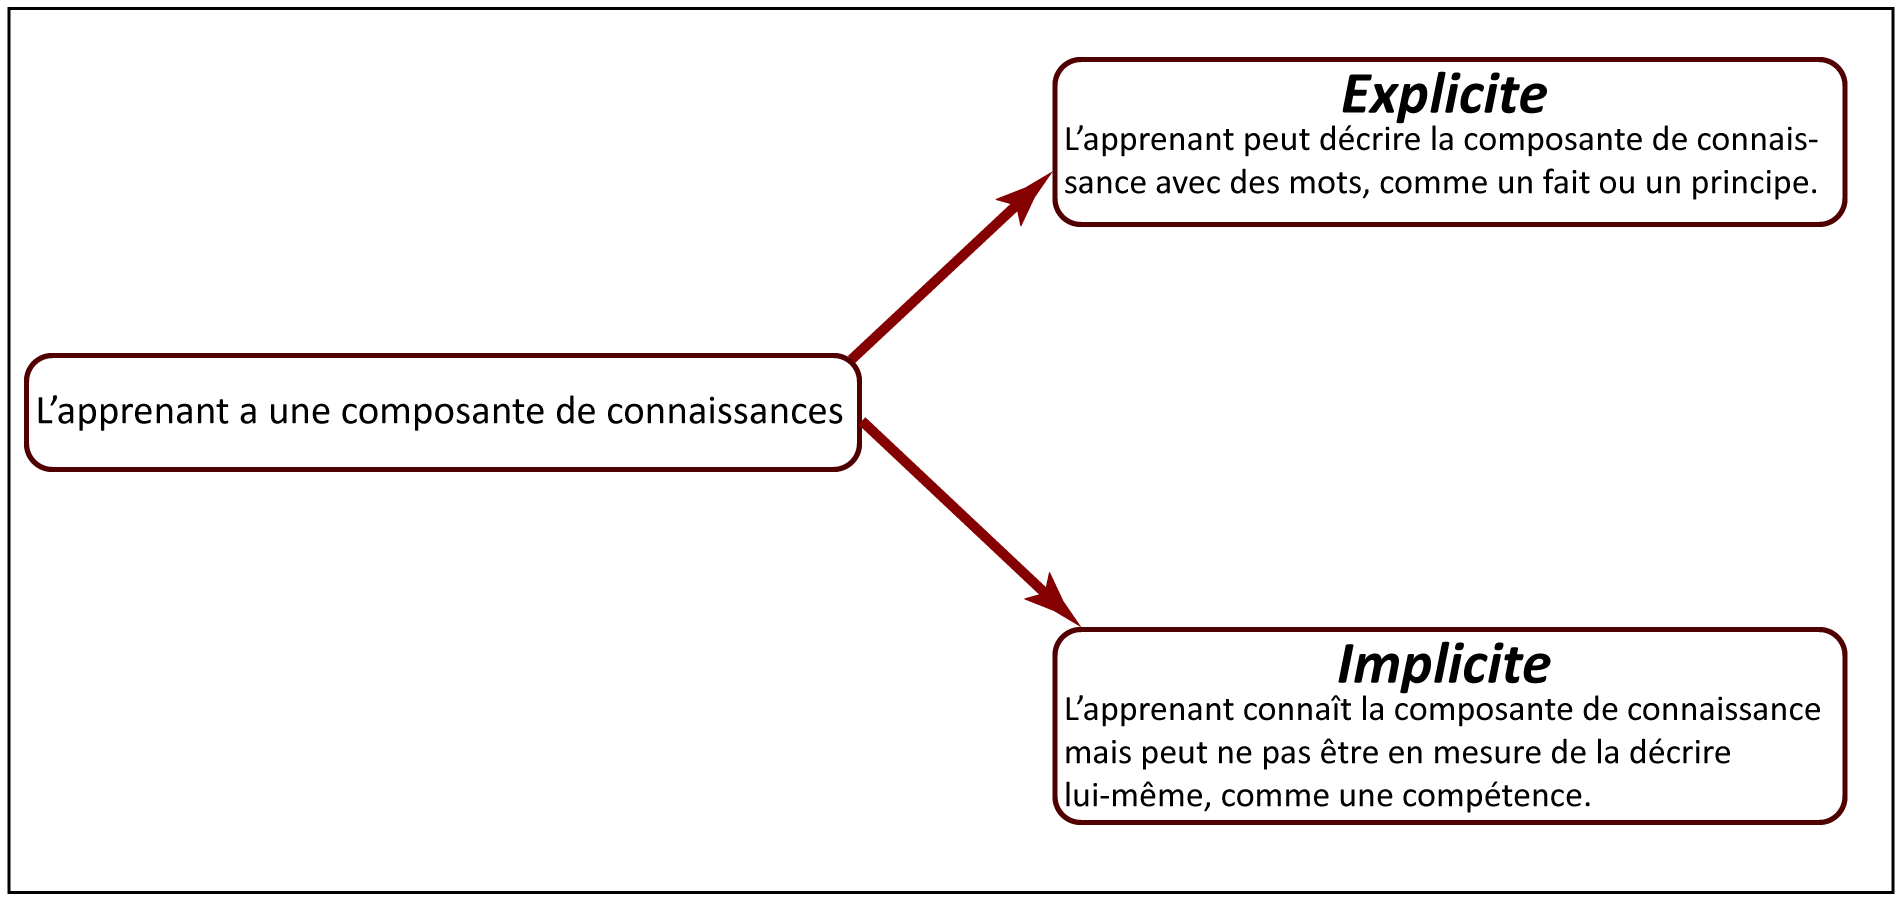
\includegraphics[width=\textwidth]{images/chapitre3/Knowledge_component.png}
	\end{center}
\caption{Knowledge Component}
\label{knowledge_component}
\end{figure}
\textbf{\underline{Exemple :}}
"Si l'angle A = 60 et (A = B, C = 60) Alors triangle équilatéral." \\
L'élève peut dessiner un triangle équilatéral sans être capable de décrire la règle. Une grande partie de ce que les apprenants de première langue savent de leur langue maternelle implique des éléments de connaissances implicites. Pertinence : la plupart des composants de connaissance explicites impliquent de nombreux composants de connaissance tacites (compétences innées ou acquises, le savoir-faire et l'expérience). La réponse et la fonctionnalité sont liées par la composante de connaissance, où les deux peuvent être externes, dans le monde, comme des signaux dans un stimulus et une réponse motrice ou interne, dans l'esprit, comme des fonctionnalités inférées et un nouvel objectif\cite{vanlehn2006behavior}.

\subsection{Les types de composante de connaissance}

La composante de connaissance est une représentation mentale de : \cite{chang2006learning}

\begin{itemize}
    \item[$\bullet$] \textbf{Connaissance du domaine :} faits, concepts, principes, règles, procédures, stratégies.
    \item[$\bullet$] \textbf{Connaissances préalables :} connaissance de l'encodage des fonctionnalités.
    \item[$\bullet$] \textbf{Connaissance intégrative :} schémas ou procédures qui connectent d'autres KC.
    \item[$\bullet$] \textbf{Connaissances métacognitives :} sur les connaissances, le contrôle de l'utilisation ou l'acquisition des connaissances.
    \item[$\bullet$] \textbf{Croyances et intérêts :} ce que l'on aime, croit.
    \item[$\bullet$] \textbf{Toute représentation externe des connaissances :} (comme les descriptions de manuels ou un exemple) ou les structures cognitives génériques (mémoire de travail), soit, les paramètres continus sur les représentations des connaissances (force, niveau d'engagement, valeur implicite d'un objectif, affect) ne sont pas des composants de connaissances.
\end{itemize}

\section{Items-to-skills mapping}
\subsection{Définition}
Les compétences (Skills) déterminent le résultat d'un individu sur une tâche dans une période donnée, à savoir si le résultat obtenu par l'individu est un succès ou un échec. La tâche à laquelle un individu est évaluer peut-être une question, un exercice, ou tout autre défi qui nécessitera certaines compétences. Les systèmes de tutorat intelligent cherchent donc à mapper ces compétences aux questionnaires ou (items) afin d'amener l'apprenant à obtenir un niveau de maîtrise sur un ensemble de compétences et aussi recommander les taches ou « items » (ou exercices) les plus appropriés compte tenu de la dernière tache effectuer par l’apprenant \cite{desmarais2012mapping}. Ce « mapping » est aussi appelée Q-matrix en EDM \cite{baker2009state}.
\subsection{items-to-skills mapping Structure}
Il existe deux approches pour mapper les éléments aux compétences présentées dans la figure \ref{items_to_skills_mapping}:

\begin{figure}[H]
	\begin{center}
		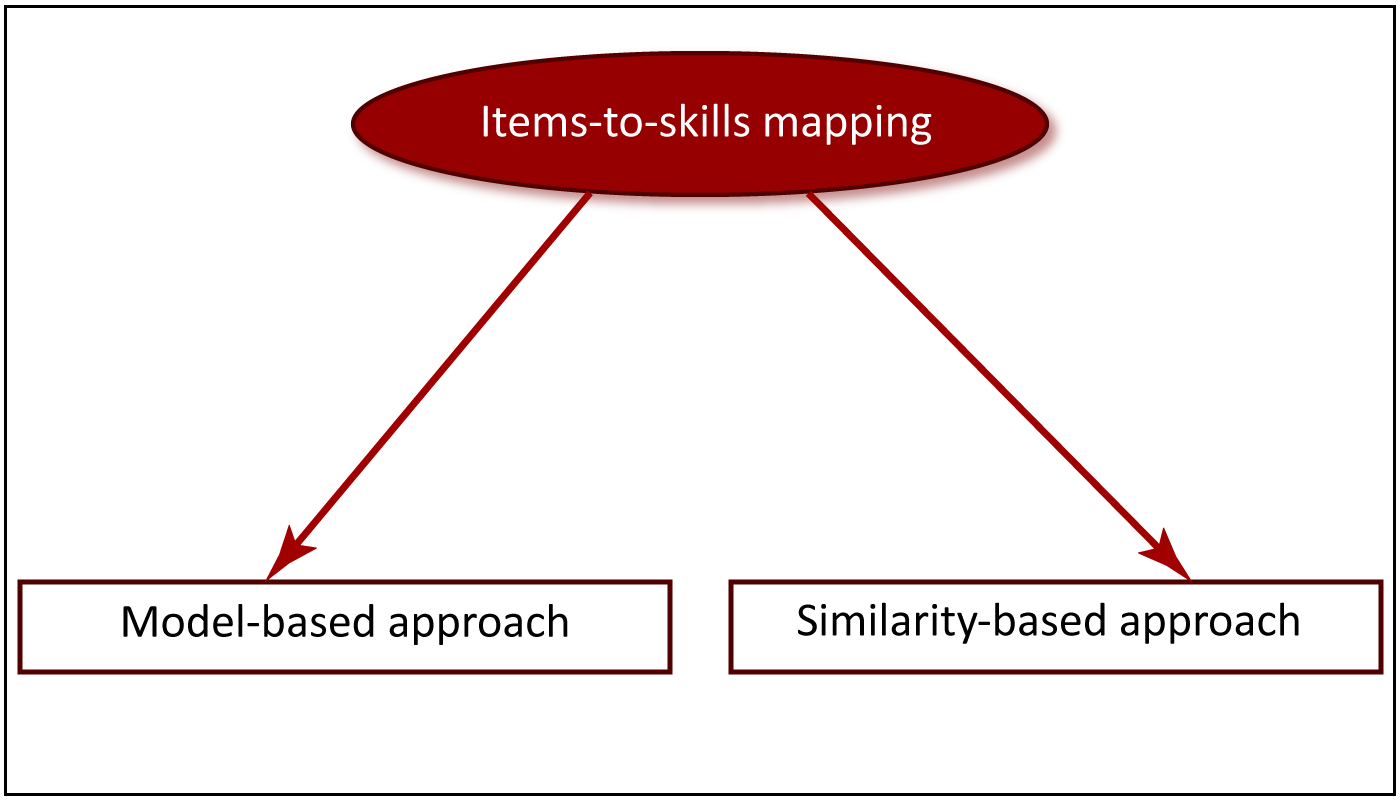
\includegraphics[width=\textwidth]{images/chapitre3/Items_mapping_structure.png}
	\end{center}
\caption{Items-to-skills mapping Structure}
\label{items_to_skills_mapping}
\end{figure}

\subsubsection{Model-Based approach}
\paragraph{Définition}
Cette approche est un modèle simplifié qui explique les données observées. Basé sur une matrice de réponses des apprenants aux éléments (ou items), le modèle prédit les réponses de l’apprenant. Le modèle attribue plusieurs compétences latentes aux apprenants et utilise le mappage des éléments aux facteurs latents correspondants. Ce type de modèle peut souvent être exprimé naturellement à l’aide de la multiplication matricielle, c’est-à-dire que l’ajustement d’un modèle conduit à une factorisation matricielle. Une fois que nous obtenons le résultat après avoir ajusté le modèle aux données, nous avons désigné les items avec la même valeur d’un facteur latent comme « similaires ». Cette approche conduit naturellement à plusieurs composantes de connaissance par compétence \cite{pelanek2018measuring}. L’approche basé sur le modèle présenté dans la figure \ref{model_based} développe un modèle de notation des utilisateurs, les algorithmes de cette catégorie adoptent une approche probabiliste en calculant la valeur attendue de la prédiction de l’utilisateur et en tenant compte des notes de l’utilisateur sur d’autres éléments \cite{item_based_recommendation_algo}. \\
Cette approche peut donc être produit par différents algorithmes d’apprentissage automatique tels que le réseau bayésien, le clustering et l’approche basée sur des règles \cite{breese2013empirical}.

\begin{figure}[H]
	\begin{center}
		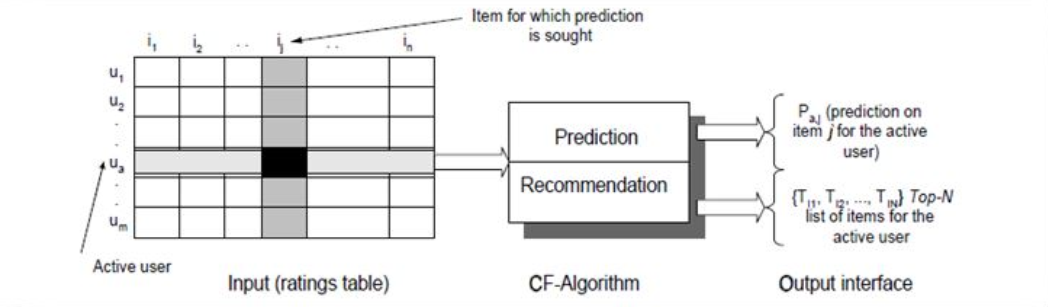
\includegraphics[width=\textwidth]{images/chapitre3/Model_based.png}
	\end{center}
\caption{Model based}
\label{model_based}
\end{figure}

Cette approche produit des composantes de connaissances différents et multiples par compétence. Le modèle est généralement calculé à l'aide d'une technique d'optimisation qui ne mène qu'à des optima locaux (par exemple, une descente de gradient). \\
Dans les systèmes recommandés, cette approche est utilisée pour la mise en œuvre du filtrage collaboratif ; elle est souvent appelée "Singular Value Decomposition" (SVD) \cite{koren2011advances}. 

\paragraph{Model Based Techniques}
Dans le contexte pédagogique, de nombreuses variantes de l'approche basée sur les modèles ont été proposées : \\

\begin{itemize}
    \item[$\bullet$] \textbf{Q-matrix :} Est une matrice binaire illustrée à la figure 4 montrant la relation entre les éléments de test et les attributs ou concepts latents ou sous-jacents (Birenbaum, et al., 1993). Les états de connaissance ont été attribués aux apprenants en fonction de leurs réponses aux tests et de la matrice q construite \cite{barnes2005q}.
\end{itemize}

\begin{figure}[H]
	\begin{center}
		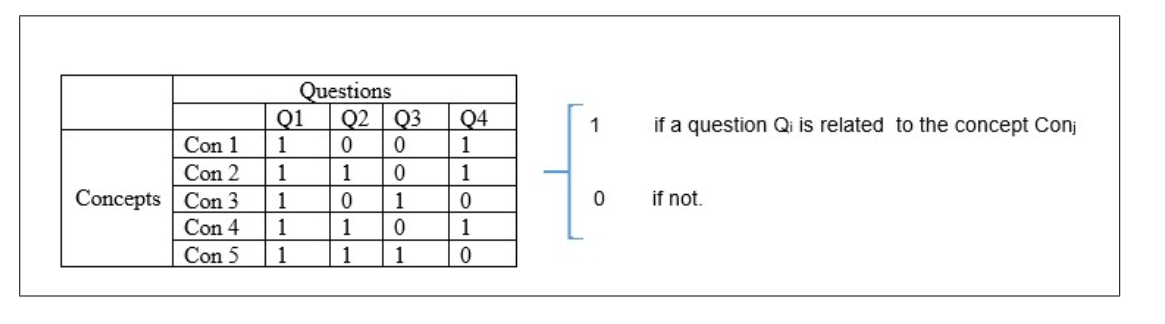
\includegraphics[width=\textwidth]{images/chapitre3/q_matrix.png}
	\end{center}
\caption{Q-matrix}
\label{q_matrix}
\end{figure}

\subsection{Similarity-based approach}
\subsubsection{Définition}
En statistiques et en mathématiques, la mesure de similarité ou la fonction de similarité est une fonction qui mesure la similarité entre deux éléments. Les valeurs de similarité entre les éléments sont quantifiées par l'observation de la performance des utilisateurs sur les éléments, qu'il s'agisse de négatif ou non \cite{nithya2017calculating}. La mesure des similarité est une étape très importante dans une analyse plus approfondie telle que le clustering des items \cite{pelanek2018measuring}.  \\
Dans cette approche, on calcule directement une mesure de similarité pour chaque paire d'éléments. Ces mesure de similarités sont ensuite utilisées pour faire le clustering, pour faire la visualisation en projetant ces éléments dans un plan a 2 ou 3 dimensions, ou pour faire d’autre analyse en essayant de récupérer les éléments les plus similaire. Cette approche est illustrée à la figure \ref{illustration_item_similarity}. 

\begin{figure}[H]
	\begin{center}
		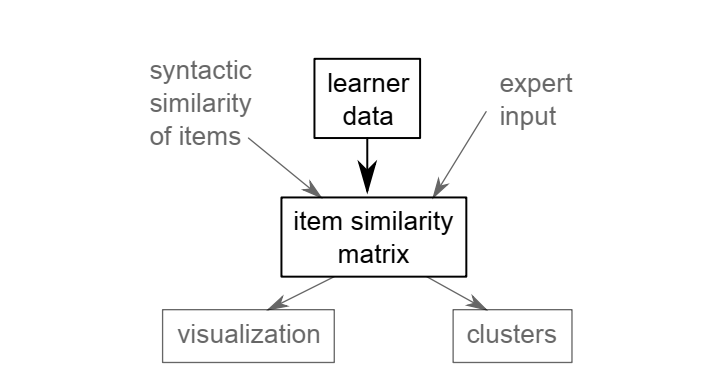
\includegraphics[scale=1]{images/chapitre3/Illustration_item_smilarity.png}
	\end{center}
\caption{Illustration de l'approche générale de l'analyse des éléments basée sur la similarité des éléments.}
\label{illustration_item_similarity}
\end{figure}

Dans l'apprentissage éducatif, la définition de la similarité des éléments a été analysée en utilisant la corrélation des réponses des apprenants et les temps de résolution des problèmes, ainsi qu'en utilisant les mauvaises réponses des apprenants. \cite{pelanek2018measuring}

\subsubsection{Processus de similarité des items (éléments)}
Une étape importante de l'approche basée sur les items consiste à calculer le degré de similarité entre chaque paire d’items, puis à sélectionner les éléments les plus similaires. Il peut être décrit comme l'opération de calcul de similarité entre deux éléments i et j, où il s'agit d'abord de définir les utilisateurs qui ont évalué ces deux éléments, puis d'appliquer une technique de calcul de similarité pour déterminer le score de similarité entre i et j. \cite{item_based_recommendation_algo} La figure \ref{calcul_application_similarity} ci-dessous montre l'approche générale du calcul et de l'application de la similarité des items.

\begin{figure}[H]
	\begin{center}
		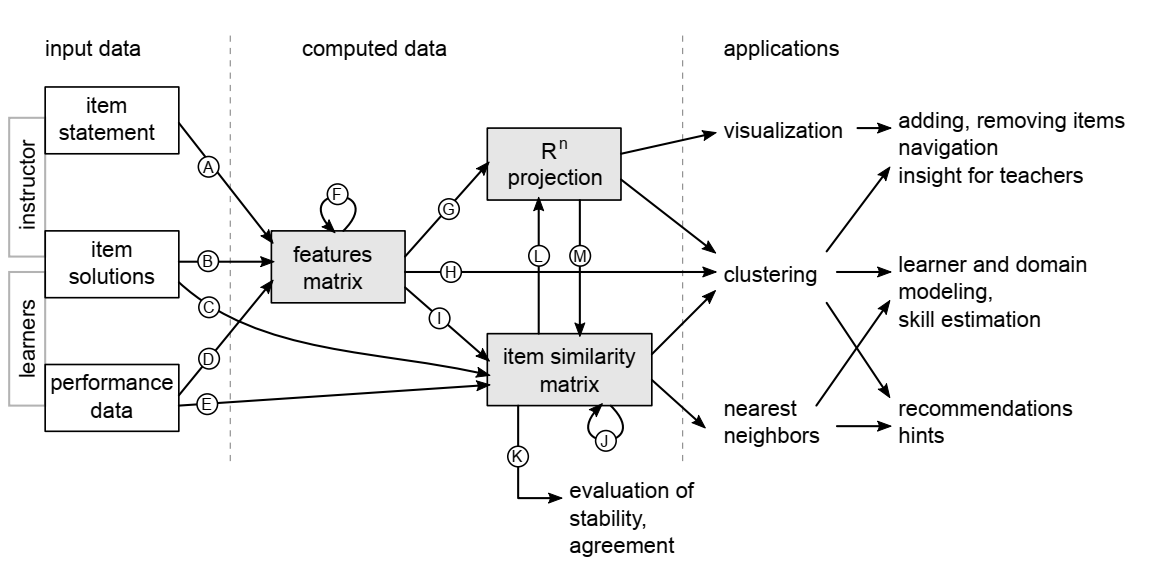
\includegraphics[width=\textwidth]{images/chapitre3/calcul_application_similarity.png}
	\end{center}
\caption{L'approche générale du calcul et de l'application de la similarité des éléments.}
\label{calcul_application_similarity}
\end{figure}

Nous allons brièvement parcourir les trois étapes input data, computed data, applications illustrées dans la figure \ref{calcul_application_similarity}. 
\paragraph{Input Data}

\begin{itemize}
    \item \underline{Item statement (Flèche A) :} Un item est la spécification de la tâche que l’apprenant doit résoudre donnée en langage naturel, ou des exemples d’entrée-sortie, et a construction de la « features matrix » nécessite d’abord un prétraitement à des items.
\end{itemize}

\begin{itemize}
    \item \underline{Item solution :} est simplement la solution donnée par l’apprenant ou la solution commune des apprenants.
\end{itemize}

\begin{itemize}
    \item \underline{Performance data :} informations sur la performance des apprenants lors de la résolution des items par exemple : exactitude de la réponse, temps de réponse, nombre d'indices utilisés et nombre de tentative faite sur un seul item.
\end{itemize}

\paragraph{Computed Data}

\begin{itemize}
    \item \underline{Features matrix :} c'est la matrice qui contient les éléments et leurs caractéristiques qui peuvent être par exemple une solution d'élément ou des mots-clés apparaissant dans une déclaration d'élément.
	\item \underline{Item similarity matrix :} est une matrice bidimensionnelle m, où m[i,j] désigne la similarité des items i et j. Le calcul de la matrice de similarité basée sur la matrice de caractéristiques (flèche I) ou sa projection dans Rn (flèche M) est une opération courante en apprentissage automatique, avec de nombreux choix disponibles, par exemple la similarité cosinus, le coefficient de corrélation de Pearson et la distance euclidienne (transformé en mesure de similarité par soustraction).
\end{itemize}

\subsubsection{Item-Similarity measures}
Pour calculer le score de similarité entres deux items, il faut tout d’abord créer la matrice d’accord entre item i et item j. Cette matrice d’accord appeler aussi matrice de confusion ou (confusion matrix en anglais) est illustrer par le tableau \ref{matrice_accord}.

\begin{table}[H]
    \centering
	\begin{tabular}{|c| c|c|}
	\hline
	 & Item i (Correct) & Item i (Incorrect)  \\ \hline
	 Item j (Correct) & a & b  \\  \hline
	 Item j (Incorrect) & c & d  \\  \hline
	\end{tabular}
	\caption{La matrice d’accord pour deux items.}
	\label{matrice_accord}
\end{table}

Où,
\begin{itemize}
	\item a : nombre d’apprenants qui ont répondu correctement à la fois à l’item i et j.
	\item b : nombre d’apprenants ayant répondu incorrectement à l’item i et l’item j correctement.
	\item c : nombre d’apprenants ayant répondu incorrectement à l’item j et l’item i correctement.
	\item d : nombre d’apprenants ayant répondu à la fois à l’item i et j de manière incorrecte.
\end{itemize}
Ensuite cette matrice d’accord est utilisée pour calculer la similarité entre l’item i et j. Les coefficients de calcule de similarité qui peuvent être utiliser sont les suivants \ref{differentes_mesures_similarité} :

\begin{table}[H]
    \centering
	\begin{tabular}{|c| c|}
	\hline
	\rowcolor{blueforest}
	\color{white} \textbf{Mesures} & \color{white} \textbf{Equation}  \\ \hline \hline
	Yule  & \(\displaystyle Sy = (ad-bc)/(ad+bc)\)   \\  \hline
	Pearson  &  \(\displaystyle Sp = (ad-bc)/\sqrt{(a+b)(a+c)(b+d)(c+d)}\) \\ \hline
	\makecell{\\Cohen \\ \\ \\}  & \makecell{\(\displaystyle Sc = (Po-Pe)/(1-Pe) \) \\ \(\displaystyle Po = (a+d)/n\) \\  \(\displaystyle Pe = ((a+b)(a+c)+(b+d)(c+d))/n^{2} \)}  \\  \hline
	Sokal  & \(\displaystyle Ss = (a+b)/(a +b +c + d)  \)   \\  \hline
	Jaccard  & \(\displaystyle Sj = a/(a+b+c) \)   \\  \hline
	Ochiai  & \(\displaystyle So = a/\sqrt{(a+b)(a+c)} \)   \\  \hline
	\end{tabular}
	\caption{Coefficients de mesures de similarités.}
	\label{differentes_mesures_similarité}
\end{table}

\section{Related work}

\section{Conclusion} 
Dans ce chapitre nous avons a introduit les concepts de base du Knowledge component, Items-to-skills mapping, en spécifiant différents coefficients de similarité qui peuvent ensuite être utilisées dans une analyse plus approfondie des relations entre les items, telles que le clustering des items ou la visualisation de ces derniers.